%====================================================%
% SEZIONE 1: Quantità di moto e impulso
%====================================================%

\begin{question}[ID=1.1, subtitle={Impulso di un calciatore sul pallone}, tags={quantità di moto, impulso}, difficulty=facile]
Un pallone da calcio di massa \(m = 0{,}4 \, \text{kg}\) si muove con una velocità di \(v = 10 \, \text{m/s}\) verso un giocatore, che lo calcia nella direzione opposta con una velocità di \(v' = 15 \, \text{m/s}\). Supponendo che l'intervallo di contatto duri \(\Delta t = 0{,}1 \, \text{s}\):
\begin{enumerate}
    \item Calcola la variazione della quantità di moto del pallone.
    \item Determina la forza impressa sul pallone dal giocatore.
\end{enumerate}
\begin{solution}
    Scegliamo positivo il verso del calcio (direzione di \(v'\)).
    La velocità iniziale del pallone è \(v_i = -10 \, \text{m/s}\), quella finale \(v_f = +15 \, \text{m/s}\).
    \begin{enumerate}
        \item Variazione della quantità di moto:
        \[
            \Delta p = m(v_f - v_i) = 0{,}4 \cdot \bigl(15 - (-10)\bigr) = 0{,}4 \cdot 25 = 10 \, \text{N·s}.
        \]
        \item Per il teorema impulso-quantità di moto, \(\vec{F}_{\text{med}} = \Delta p / \Delta t\):
        \[
            F = \frac{10}{0{,}1} = 100 \, \text{N}.
        \]
    \end{enumerate}
\end{solution}
\end{question}

%----------------------------------------------------%

\begin{question}[ID=1.2, subtitle={Impulso vettoriale su un disco di hockey}, tags={quantità di moto, impulso, variazione vettoriale}, difficulty=media]
Un disco di hockey di massa \(0{,}16 \, \text{kg}\) scivola su un piano orizzontale privo di attrito con velocità \(\vec{v}_i = (8\,\hat{\imath} + 3\,\hat{\jmath}) \, \text{m/s}\).
Viene colpito da una mazza che imprime un impulso \(\vec{J} = (-1{,}6\,\hat{\imath} + 0{,}8\,\hat{\jmath}) \, \text{N·s}\).
\begin{enumerate}
    \item Determina la velocità finale del disco.
    \item Calcola il modulo della variazione di quantità di moto.
    \item Qual è l'angolo tra le direzioni iniziale e finale della velocità?
\end{enumerate}
\begin{solution}
    \begin{enumerate}
        \item La velocità finale si ottiene da \(\vec{J} = m\Delta\vec{v}\):
        \[
            \vec{v}_f = \vec{v}_i + \frac{\vec{J}}{m}
            = (8\,\hat{\imath}+3\,\hat{\jmath}) + \frac{-1{,}6\,\hat{\imath}+0{,}8\,\hat{\jmath}}{0{,}16}
            = (8-10)\,\hat{\imath} + (3+5)\,\hat{\jmath}
            = (-2\,\hat{\imath} + 8\,\hat{\jmath}) \, \text{m/s}.
        \]
        \item Il modulo della variazione di quantità di moto coincide con \(|\vec{J}|\):
        \[
            |\Delta\vec{p}| = |\vec{J}| = \sqrt{(-1{,}6)^2 + 0{,}8^2} = \sqrt{2{,}56 + 0{,}64} = \sqrt{3{,}2} \approx 1{,}79 \, \text{N·s}.
        \]
        \item L'angolo tra \(\vec{v}_i\) e \(\vec{v}_f\):
        \[
            \cos\theta = \frac{\vec{v}_i \cdot \vec{v}_f}{|\vec{v}_i||\vec{v}_f|}
            = \frac{(8)(-2)+(3)(8)}{\sqrt{73}\cdot\sqrt{68}}
            = \frac{8}{\sqrt{4964}} \approx \frac{8}{70{,}46} \approx 0{,}114,
        \]
        \[
            \theta \approx \arccos(0{,}114) \approx 83{,}5^\circ.
        \]
    \end{enumerate}
\end{solution}
\end{question}

%----------------------------------------------------%

\begin{question}[ID=1.3, subtitle={Impulso da una forza triangolare nel tempo}, tags={impulso, forza variabile, grafico forza-tempo}, difficulty=media]
Un corpo di massa \(2 \, \text{kg}\) riceve una forza variabile nel tempo descritta dal seguente profilo: la forza cresce linearmente da \(0\) a \(10 \, \text{N}\) nei primi \(0{,}2 \, \text{s}\), poi decresce linearmente a \(0\) in altri \(0{,}2 \, \text{s}\).
\begin{enumerate}
    \item Determina l'impulso totale.
    \item Calcola la variazione di velocità del corpo.
\end{enumerate}
\begin{solution}
    \begin{enumerate}
        \item L'impulso è uguale all'area sotto il grafico \(F(t)\): un triangolo isoscele di base \(0{,}4 \, \text{s}\) e altezza \(10 \, \text{N}\):
        \[
            J = \frac{1}{2} \cdot 0{,}4 \cdot 10 = 2 \, \text{N·s}.
        \]
        \item Per il teorema impulso-quantità di moto:
        \[
            \Delta v = \frac{J}{m} = \frac{2}{2} = 1 \, \text{m/s}.
        \]
    \end{enumerate}
\end{solution}
\end{question}

%----------------------------------------------------%

\begin{question}[ID=1.4, subtitle={Rimbalzo obliquo su parete liscia}, tags={quantità di moto, urto con parete}, difficulty=difficile]
Una pallina di massa \(0{,}05 \, \text{kg}\) colpisce una parete liscia con velocità \(10 \, \text{m/s}\) formando un angolo di \(30^\circ\) con la normale alla parete, e rimbalza con la stessa velocità (urto elastico).
\begin{enumerate}
    \item Calcola la variazione vettoriale della quantità di moto.
    \item Determina la forza media esercitata dalla parete se il contatto dura \(0{,}01 \, \text{s}\).
\end{enumerate}
\begin{solution}
    \begin{enumerate}
        \item Prendiamo \(x\) perpendicolare alla parete (verso di incidenza) e \(y\) parallela.
        La componente tangenziale è invariata; la componente normale si inverte:
        \[
            v_x^{(i)} = v\cos30^\circ = 10 \cdot \tfrac{\sqrt{3}}{2} = 5\sqrt{3} \, \text{m/s},
            \qquad v_y^{(i)} = v\sin30^\circ = 5 \, \text{m/s}.
        \]
        \[
            \Delta v_x = -2v\cos30^\circ = -10\sqrt{3} \, \text{m/s}, \qquad \Delta v_y = 0.
        \]
        \[
            |\Delta\vec{p}| = m \cdot 2v\cos30^\circ = 0{,}05 \cdot 10\sqrt{3} = 0{,}5\sqrt{3} \approx 0{,}866 \, \text{N·s}.
        \]
        \item Forza media (diretta perpendicolarmente alla parete, verso l'esterno):
        \[
            F = \frac{|\Delta\vec{p}|}{\Delta t} = \frac{0{,}866}{0{,}01} = 86{,}6 \, \text{N}.
        \]
    \end{enumerate}
\end{solution}
\end{question}

%----------------------------------------------------%

\begin{question}[ID=1.5, subtitle={Variazione di velocità con impulso e attrito}, tags={impulso, attrito}, difficulty=difficile]
Un blocco di massa \(m = 1 \, \text{kg}\) scivola su un piano orizzontale con velocità iniziale \(5 \, \text{m/s}\). Dopo \(0{,}4 \, \text{s}\) inizia ad agire una forza costante \(F = 6 \, \text{N}\) contraria al moto per \(0{,}3 \, \text{s}\); dopodiché il blocco scivola su una superficie con coefficiente di attrito dinamico \(\mu = 0{,}2\).
\begin{enumerate}
    \item Calcola la velocità del blocco subito dopo la fase di impulso.
    \item Determina il tempo necessario al blocco per fermarsi dopo la fase di impulso.
\end{enumerate}
\begin{solution}
    \begin{enumerate}
        \item Nella fase di impulso \(\vec{J} = -F\Delta t\) (opposto al moto):
        \[
            \Delta v = -\frac{F \Delta t}{m} = -\frac{6 \cdot 0{,}3}{1} = -1{,}8 \, \text{m/s}.
        \]
        La velocità dopo l'impulso:
        \[
            v_1 = 5 - 1{,}8 = 3{,}2 \, \text{m/s}.
        \]
        \item Decelerazione per attrito:
        \[
            a = -\mu g = -0{,}2 \cdot 9{,}81 = -1{,}962 \, \text{m/s}^2.
        \]
        Tempo per fermarsi:
        \[
            t = \frac{v_1}{|a|} = \frac{3{,}2}{1{,}962} \approx 1{,}63 \, \text{s}.
        \]
    \end{enumerate}
\end{solution}
\end{question}

%----------------------------------------------------%

\begin{question}[ID=1.6, subtitle={Velocità di un pallone dopo un calcio}, tags={impulso}, difficulty=media]
Un pallone da calcio di massa \(m = 0{,}45 \, \text{kg}\) è inizialmente fermo. Viene colpito da un giocatore con una forza media di \(F = 120 \, \text{N}\) per un tempo \(\Delta t = 0{,}05 \, \text{s}\).
\begin{enumerate}
    \item Calcola l'impulso ricevuto dal pallone.
    \item Qual è la velocità finale del pallone subito dopo il calcio?
\end{enumerate}
\begin{solution}
    \begin{enumerate}
        \item Impulso ricevuto:
        \[
            J = F \cdot \Delta t = 120 \cdot 0{,}05 = 6 \, \text{N·s}.
        \]
        \item Poiché il pallone era fermo, \(\Delta p = J\):
        \[
            v_f = \frac{J}{m} = \frac{6}{0{,}45} \approx 13{,}3 \, \text{m/s}.
        \]
    \end{enumerate}
\end{solution}
\end{question}

%====================================================%
% SEZIONE 2: Urti elastici
%====================================================%

\begin{question}[ID=2.1, subtitle={Velocità finali in un urto elastico 1D}, tags={urti elastici, energia cinetica}, difficulty=facile]
Una pallina di massa \(m_1 = 4 \, \text{kg}\) si muove con velocità \(v_{1i} = 6 \, \text{m/s}\) verso destra e colpisce una seconda pallina di massa \(m_2 = 6 \, \text{kg}\), che si muove verso sinistra con velocità \(v_{2i} = -4 \, \text{m/s}\). L'urto è elastico e avviene lungo una linea retta.
\begin{enumerate}
    \item Quali sono le velocità finali \(v_{1f}\) e \(v_{2f}\) delle due palline dopo l'urto?
    \item Calcola l'energia cinetica del sistema prima e dopo l'urto e verifica la conservazione.
\end{enumerate}
\begin{solution}
    \begin{enumerate}
        \item Formule per urto elastico 1D:
        \[
            v_{1f} = \frac{m_1 - m_2}{m_1 + m_2}v_{1i} + \frac{2m_2}{m_1+m_2}v_{2i}
            = \frac{-2}{10}(6) + \frac{12}{10}(-4) = -1{,}2 - 4{,}8 = -6 \, \text{m/s}.
        \]
        \[
            v_{2f} = \frac{2m_1}{m_1+m_2}v_{1i} + \frac{m_2 - m_1}{m_1+m_2}v_{2i}
            = \frac{8}{10}(6) + \frac{2}{10}(-4) = 4{,}8 - 0{,}8 = 4 \, \text{m/s}.
        \]
        \item Energia cinetica prima:
        \[
            E_{ki} = \tfrac{1}{2}(4)(6^2) + \tfrac{1}{2}(6)(4^2) = 72 + 48 = 120 \, \text{J}.
        \]
        Energia cinetica dopo:
        \[
            E_{kf} = \tfrac{1}{2}(4)(6^2) + \tfrac{1}{2}(6)(4^2) = 72 + 48 = 120 \, \text{J}.
        \]
        L'energia cinetica si conserva: \(E_{ki} = E_{kf} = 120 \, \text{J}\). \checkmark
    \end{enumerate}
\end{solution}
\end{question}

%----------------------------------------------------%

\begin{question}[ID=2.2, subtitle={Urto elastico tra due carrelli su binario}, tags={urti elastici, sistema isolato}, difficulty=media]
Due carrelli su un binario privo d'attrito hanno masse \(m_1 = 0{,}8 \, \text{kg}\) e \(m_2 = 1{,}2 \, \text{kg}\). Il primo si muove a \(v_{1i} = 3 \, \text{m/s}\) verso destra, il secondo a \(v_{2i} = 1 \, \text{m/s}\) verso sinistra. L'urto è elastico.
\begin{enumerate}
    \item Calcola le velocità finali dei due carrelli.
    \item Verifica la conservazione dell'energia cinetica.
\end{enumerate}
\begin{solution}
    \begin{enumerate}
        \item Poniamo positivo verso destra, quindi \(v_{2i} = -1 \, \text{m/s}\):
        \[
            v_{1f} = \frac{m_1 - m_2}{m_1+m_2}v_{1i} + \frac{2m_2}{m_1+m_2}v_{2i}
            = \frac{-0{,}4}{2}(3) + \frac{2{,}4}{2}(-1) = -0{,}6 - 1{,}2 = -1{,}8 \, \text{m/s}.
        \]
        \[
            v_{2f} = \frac{2m_1}{m_1+m_2}v_{1i} + \frac{m_2-m_1}{m_1+m_2}v_{2i}
            = \frac{1{,}6}{2}(3) + \frac{0{,}4}{2}(-1) = 2{,}4 - 0{,}2 = 2{,}2 \, \text{m/s}.
        \]
        \item Energia cinetica prima: \(E_{ki} = \tfrac{1}{2}(0{,}8)(9) + \tfrac{1}{2}(1{,}2)(1) = 3{,}6 + 0{,}6 = 4{,}2 \, \text{J}\).

        Energia cinetica dopo: \(E_{kf} = \tfrac{1}{2}(0{,}8)(3{,}24) + \tfrac{1}{2}(1{,}2)(4{,}84) = 1{,}296 + 2{,}904 = 4{,}2 \, \text{J}\). \checkmark
    \end{enumerate}
\end{solution}
\end{question}

%----------------------------------------------------%

\begin{question}[ID=2.3, subtitle={Determinazione della massa in un urto elastico}, tags={urti elastici, riflessione}, difficulty=difficile]
Un corpo di massa \(m_1 = 1 \, \text{kg}\) si muove a \(5 \, \text{m/s}\) e urta elasticamente un corpo fermo di massa \(m_2\). Dopo l'urto, il primo corpo si ferma completamente. Determina:
\begin{enumerate}
    \item Il valore di \(m_2\).
    \item La velocità finale di \(m_2\).
\end{enumerate}
\begin{solution}
    \begin{enumerate}
        \item Se \(v_{1f} = 0\), dalla formula delle velocità finali elastiche:
        \[
            v_{1f} = \frac{m_1 - m_2}{m_1 + m_2} v_{1i} = 0 \implies m_1 = m_2.
        \]
        Quindi \(m_2 = 1 \, \text{kg}\).
        \item Dalla conservazione della quantità di moto:
        \[
            m_1 v_{1i} = m_2 v_{2f} \implies v_{2f} = \frac{m_1}{m_2} v_{1i} = 5 \, \text{m/s}.
        \]
    \end{enumerate}
\end{solution}
\end{question}

%----------------------------------------------------%

\begin{question}[ID=2.4, subtitle={Urti elastici sequenziali tra tre sfere identiche}, tags={urti elastici, energia, sistema a tre corpi}, difficulty=difficile]
Tre sfere identiche su un piano privo d'attrito sono disposte in fila. La prima si muove a \(6 \, \text{m/s}\); le altre due sono ferme. Ogni urto è elastico e avviene solo tra due sfere per volta.
\begin{enumerate}
    \item Determina la velocità di ciascuna sfera dopo tutti gli urti.
\end{enumerate}
\begin{solution}
    \begin{enumerate}
        \item Per due sfere identiche in urto elastico \(1\)D, il corpo che si muove si ferma e l'altro parte con la stessa velocità (scambio completo).

        \textbf{Primo urto} (sfera~1 colpisce sfera~2):
        sfera~1 \(\to 0\), sfera~2 \(\to 6 \, \text{m/s}\).

        \textbf{Secondo urto} (sfera~2 colpisce sfera~3):
        sfera~2 \(\to 0\), sfera~3 \(\to 6 \, \text{m/s}\).

        \textbf{Risultato finale}: sfera~1 e sfera~2 ferme; sfera~3 si muove a \(6 \, \text{m/s}\).
    \end{enumerate}
\end{solution}
\end{question}

%----------------------------------------------------%

\begin{question}[ID=2.5, subtitle={Urto elastico tra particelle identiche nel centro di massa}, tags={urti elastici, laboratorio di riferimento}, difficulty=difficile]
Nel laboratorio, una particella di massa \(m\) e velocità \(v\) urta elasticamente una seconda particella identica inizialmente ferma.
\begin{enumerate}
    \item Trova le velocità delle due particelle nel sistema del centro di massa (CM) prima e dopo l'urto.
    \item Determina le velocità e l'angolo di deviazione nel laboratorio per un urto frontale nel sistema del CM.
\end{enumerate}
\begin{solution}
    \begin{enumerate}
        \item Velocità del CM: \(v_{CM} = v/2\).

        Nel sistema CM prima dell'urto:
        \[
            u_1 = v - v_{CM} = \tfrac{v}{2}, \qquad u_2 = 0 - v_{CM} = -\tfrac{v}{2}.
        \]
        In un urto elastico 1D nel CM le velocità si invertono:
        \[
            u_1' = -\tfrac{v}{2}, \qquad u_2' = +\tfrac{v}{2}.
        \]
        \item Riportando nel laboratorio (aggiungendo \(v_{CM} = v/2\)):
        \[
            v_{1f} = u_1' + v_{CM} = -\tfrac{v}{2} + \tfrac{v}{2} = 0.
        \]
        \[
            v_{2f} = u_2' + v_{CM} = +\tfrac{v}{2} + \tfrac{v}{2} = v.
        \]
        La prima particella si ferma e la seconda acquisisce tutta la velocità iniziale (deviazione \(0^\circ\), moto in avanti). Questo è coerente con il risultato dell'esercizio 2.3 per masse identiche.
    \end{enumerate}
\end{solution}
\end{question}

%====================================================%
% SEZIONE 3: Urti anelastici
%====================================================%

\begin{question}[ID=3.1, subtitle={Urto completamente anelastico tra due vagoni ferroviari}, tags={urti anelastici, energia cinetica}, difficulty=facile]
Un vagone ferroviario di massa \(m_1 = 8000 \, \text{kg}\) viaggia con velocità \(v_1 = 20 \, \text{m/s}\) e colpisce un secondo vagone fermo identico al primo. Dopo l'urto i due vagoni si muovono insieme.

\begin{wrapfigure}{r}{0.3\textwidth}
    \centering
    \vspace{-20pt}
    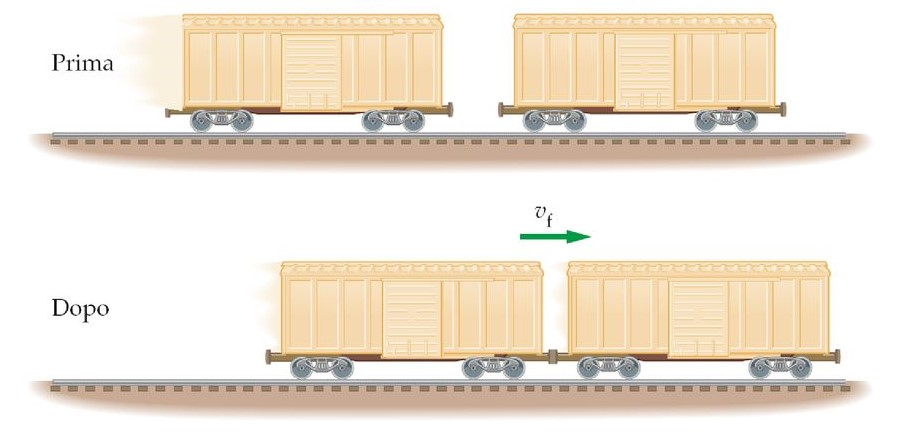
\includegraphics[width=0.28\textwidth]{images/vagoni}
\end{wrapfigure}

\begin{enumerate}
    \item Qual è la velocità comune dei veicoli subito dopo l'urto?
    \item Calcola la perdita di energia cinetica.
\end{enumerate}
\begin{solution}
    \begin{enumerate}
        \item Conservazione della quantità di moto:
        \[
            m_1 v_1 = (m_1 + m_2) v_f \implies v_f = \frac{8000 \cdot 20}{16000} = 10 \, \text{m/s}.
        \]
        \item Energie cinetiche:
        \[
            E_{ki} = \tfrac{1}{2}(8000)(20^2) = 1{,}60 \times 10^6 \, \text{J},
        \]
        \[
            E_{kf} = \tfrac{1}{2}(16000)(10^2) = 8{,}00 \times 10^5 \, \text{J}.
        \]
        Perdita di energia:
        \[
            \Delta E_k = E_{ki} - E_{kf} = 1{,}60 \times 10^6 - 8{,}00 \times 10^5 = 8{,}00 \times 10^5 \, \text{J} = 800 \, \text{kJ}.
        \]
    \end{enumerate}
\end{solution}
\end{question}

%----------------------------------------------------%

\begin{question}[ID=3.2, subtitle={Pendolo balistico: altezza raggiunta dal blocco}, tags={urti anelastici, sistema chiuso}, difficulty=media]
Un proiettile di massa \(m_p = 0{,}02 \, \text{kg}\) si conficca in un blocco di massa \(M = 2 \, \text{kg}\) sospeso a un filo. La velocità iniziale del proiettile è \(v_0 = 300 \, \text{m/s}\).
\begin{enumerate}
    \item Determina la velocità del sistema subito dopo l'urto.
    \item Calcola di quanto si solleva il blocco.
\end{enumerate}
\begin{solution}
    \begin{enumerate}
        \item Conservazione della quantità di moto nell'urto:
        \[
            v_f = \frac{m_p \, v_0}{m_p + M} = \frac{0{,}02 \cdot 300}{2{,}02} = \frac{6}{2{,}02} \approx 2{,}97 \, \text{m/s}.
        \]
        \item Conservazione dell'energia meccanica dopo l'urto (\(E_k \to E_p\)):
        \[
            h = \frac{v_f^2}{2g} = \frac{(2{,}97)^2}{2 \cdot 9{,}81} = \frac{8{,}82}{19{,}62} \approx 0{,}45 \, \text{m}.
        \]
    \end{enumerate}
\end{solution}
\end{question}

%----------------------------------------------------%

\begin{question}[ID=3.3, subtitle={Proiettile che si conficca nel bordo di un disco rotante}, tags={urti anelastici, momento angolare}, difficulty=difficile]
Un proiettile di massa \(m = 0{,}01 \, \text{kg}\) e velocità \(v_0 = 200 \, \text{m/s}\) si conficca nel bordo di un disco uniforme di massa \(M = 2 \, \text{kg}\) e raggio \(R = 0{,}2 \, \text{m}\), inizialmente fermo e libero di ruotare attorno al suo centro.
\begin{enumerate}
    \item Determina la velocità angolare del disco dopo l'urto.
    \item Calcola la perdita di energia cinetica.
\end{enumerate}
\begin{solution}
    \begin{enumerate}
        \item Conservazione del momento angolare rispetto al centro del disco:
        \[
            L_i = m v_0 R, \qquad L_f = I_{\text{tot}}\,\omega,
        \]
        \[
            I_{\text{tot}} = \tfrac{1}{2}MR^2 + mR^2 = R^2\!\left(\tfrac{M}{2} + m\right) = (0{,}04)\left(1 + 0{,}01\right) = 0{,}0404 \, \text{kg·m}^2.
        \]
        \[
            \omega = \frac{m v_0 R}{I_{\text{tot}}} = \frac{0{,}01 \cdot 200 \cdot 0{,}2}{0{,}0404} = \frac{0{,}4}{0{,}0404} \approx 9{,}9 \, \text{rad/s}.
        \]
        \item Energia cinetica iniziale e finale:
        \[
            E_{ki} = \tfrac{1}{2}m v_0^2 = \tfrac{1}{2}(0{,}01)(200)^2 = 200 \, \text{J}.
        \]
        \[
            E_{kf} = \tfrac{1}{2} I_{\text{tot}}\,\omega^2 = \tfrac{1}{2}(0{,}0404)(9{,}9)^2 \approx 1{,}98 \, \text{J}.
        \]
        \[
            \Delta E_k = 200 - 1{,}98 \approx 198 \, \text{J}.
        \]
    \end{enumerate}
\end{solution}
\end{question}

%----------------------------------------------------%

\begin{question}[ID=3.4, subtitle={Velocità comune e percentuale di energia dissipata}, tags={urti anelastici, energia dissipata}, difficulty=difficile]
Due automobili di masse \(m_1 = 900 \, \text{kg}\) e \(m_2 = 1200 \, \text{kg}\) si muovono nella stessa direzione rispettivamente a \(25 \, \text{m/s}\) e \(15 \, \text{m/s}\), e si agganciano dopo la collisione.
\begin{enumerate}
    \item Trova la velocità comune dopo l'urto.
    \item Calcola la percentuale di energia cinetica dissipata.
\end{enumerate}
\begin{solution}
    \begin{enumerate}
        \item Conservazione della quantità di moto:
        \[
            v_f = \frac{m_1 v_1 + m_2 v_2}{m_1+m_2} = \frac{900 \cdot 25 + 1200 \cdot 15}{2100} = \frac{22500 + 18000}{2100} = \frac{40500}{2100} \approx 19{,}3 \, \text{m/s}.
        \]
        \item Energia cinetica prima e dopo:
        \[
            E_{ki} = \tfrac{1}{2}(900)(625) + \tfrac{1}{2}(1200)(225) = 281250 + 135000 = 416250 \, \text{J}.
        \]
        \[
            E_{kf} = \tfrac{1}{2}(2100)(19{,}3)^2 \approx \tfrac{1}{2}(2100)(372{,}5) \approx 390750 \, \text{J}.
        \]
        \[
            \eta = \frac{E_{ki} - E_{kf}}{E_{ki}} \times 100 \approx \frac{25500}{416250} \times 100 \approx 6{,}1\%.
        \]
    \end{enumerate}
\end{solution}
\end{question}

%----------------------------------------------------%

\begin{question}[ID=3.5, subtitle={Urti anelastici sequenziali tra tre vagoni}, tags={urti anelastici, sistemi complessi}, difficulty=difficile]
Un vagone di massa \(m_1 = 5000 \, \text{kg}\) in movimento a \(5 \, \text{m/s}\) urta e si aggancia con un secondo vagone fermo di massa \(m_2 = 3000 \, \text{kg}\). Il sistema risultante urta successivamente un terzo vagone fermo di massa \(m_3 = 2000 \, \text{kg}\) e si aggancia ad esso.
\begin{enumerate}
    \item Determina la velocità finale complessiva.
    \item Calcola la perdita complessiva di energia cinetica.
\end{enumerate}
\begin{solution}
    \begin{enumerate}
        \item \textbf{Primo urto} (\(m_1\) su \(m_2\)):
        \[
            v_1 = \frac{5000 \cdot 5}{5000 + 3000} = \frac{25000}{8000} = 3{,}125 \, \text{m/s}.
        \]
        \textbf{Secondo urto} (\(m_1 + m_2\) su \(m_3\)):
        \[
            v_f = \frac{8000 \cdot 3{,}125}{8000 + 2000} = \frac{25000}{10000} = 2{,}5 \, \text{m/s}.
        \]
        \item Energia cinetica iniziale e finale:
        \[
            E_{ki} = \tfrac{1}{2}(5000)(5^2) = 62500 \, \text{J}.
        \]
        \[
            E_{kf} = \tfrac{1}{2}(10000)(2{,}5^2) = 31250 \, \text{J}.
        \]
        \[
            \Delta E_k = 62500 - 31250 = 31250 \, \text{J} = 31{,}25 \, \text{kJ}.
        \]
    \end{enumerate}
\end{solution}
\end{question}

%====================================================%
% SEZIONE 4: Urti nel piano
%====================================================%

\begin{question}[ID=4.1, subtitle={Urto elastico 2D tra palle da biliardo di massa uguale}, tags={urti nel piano, energia cinetica}, difficulty=media]
In una partita a biliardo, una palla di massa \(m = 100 \, \text{g}\) si muove con velocità \(v_{1i} = 4 \, \text{m/s}\) lungo l'asse \(x\) e colpisce una seconda palla ferma di uguale massa. Dopo l'urto elastico, la prima si muove con un angolo di \(30^\circ\) rispetto all'asse \(x\).

\begin{wrapfigure}{r}{0.3\textwidth}
    \centering
    \vspace{-20pt}
    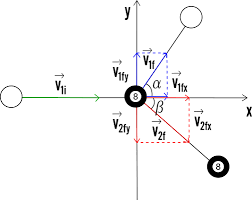
\includegraphics[width=0.28\textwidth]{images/biliardo.png}
\end{wrapfigure}

\begin{enumerate}
    \item Qual è l'angolo con cui si muove la seconda palla rispetto all'asse \(x\)?
    \item Calcola le velocità delle due palle dopo l'urto.
\end{enumerate}
\begin{solution}
    \begin{enumerate}
        \item Per un urto elastico tra masse uguali, i vettori velocità finali sono \textbf{perpendicolari}. Se la prima si muove a \(30^\circ\), la seconda si muove a:
        \[
            \theta_2 = 30^\circ - 90^\circ = -60^\circ \quad \text{(ossia } 60^\circ \text{ sotto l'asse } x\text{)}.
        \]
        \item Dalla conservazione dell'energia e della quantità di moto lungo \(y\):
        \[
            0 = v_{1f}\sin30^\circ - v_{2f}\sin60^\circ \implies \frac{v_{1f}}{2} = \frac{v_{2f}\sqrt{3}}{2} \implies v_{1f} = v_{2f}\sqrt{3}.
        \]
        Conservazione dell'energia (\(m\) si semplifica):
        \[
            v_{1f}^2 + v_{2f}^2 = v_{1i}^2 = 16 \implies 3v_{2f}^2 + v_{2f}^2 = 16 \implies v_{2f} = 2 \, \text{m/s}.
        \]
        \[
            v_{1f} = 2\sqrt{3} \approx 3{,}46 \, \text{m/s}.
        \]
    \end{enumerate}
\end{solution}
\end{question}

%----------------------------------------------------%

\begin{question}[ID=4.2, subtitle={Velocità finali in urto elastico piano tra sfere identiche}, tags={urti nel piano, conservazione vettoriale}, difficulty=media]
Due sfere identiche di massa \(0{,}1 \, \text{kg}\) si urtano elasticamente. La prima si muove con \(4 \, \text{m/s}\) lungo l'asse \(x\), la seconda con \(3 \, \text{m/s}\) lungo \(y\). Dopo l'urto, la seconda si muove a \(45^\circ\) rispetto all'asse \(x\).
\begin{enumerate}
    \item Determina le velocità finali delle due sfere.
\end{enumerate}
\begin{solution}
    \begin{enumerate}
        \item Sia \(v_{2f}\) il modulo della velocità finale della sfera 2, con direzione \(45^\circ\):
        \(\vec{v}_{2f} = \frac{v_{2f}}{\sqrt{2}}(\hat{\imath}+\hat{\jmath})\).

        Conservazione della quantità di moto (le masse si semplificano):
        \[
            v_{1fx} = 4 - \frac{v_{2f}}{\sqrt{2}}, \qquad v_{1fy} = 3 - \frac{v_{2f}}{\sqrt{2}}.
        \]
        Conservazione dell'energia:
        \[
            v_{1fx}^2 + v_{1fy}^2 + v_{2f}^2 = 4^2 + 3^2 = 25.
        \]
        Sostituendo:
        \[
            \left(4 - \frac{v_{2f}}{\sqrt{2}}\right)^2 + \left(3 - \frac{v_{2f}}{\sqrt{2}}\right)^2 + v_{2f}^2 = 25,
        \]
        \[
            25 - \frac{14\,v_{2f}}{\sqrt{2}} + v_{2f}^2 + v_{2f}^2 = 25 \implies 2v_{2f}^2 = \frac{14\,v_{2f}}{\sqrt{2}},
        \]
        \[
            v_{2f} = \frac{7}{\sqrt{2}} = \frac{7\sqrt{2}}{2} \approx 4{,}95 \, \text{m/s}.
        \]
        Le componenti della sfera 1:
        \[
            v_{1fx} = 4 - \tfrac{7}{2} = 0{,}5 \, \text{m/s}, \qquad v_{1fy} = 3 - \tfrac{7}{2} = -0{,}5 \, \text{m/s},
        \]
        \[
            v_{1f} = \sqrt{0{,}5^2 + 0{,}5^2} = \frac{1}{\sqrt{2}} \approx 0{,}71 \, \text{m/s} \quad \text{a } -45^\circ \text{ rispetto a } x.
        \]
    \end{enumerate}
\end{solution}
\end{question}

%----------------------------------------------------%

\begin{question}[ID=4.3, subtitle={Riflessione elastica su parete inclinata di 45°}, tags={urti nel piano, energia cinetica}, difficulty=difficile]
Una pallina di massa \(m\) si muove orizzontalmente con \(v = 6 \, \text{m/s}\) e urta elasticamente una parete liscia inclinata di \(45^\circ\) rispetto alla verticale.
\begin{enumerate}
    \item Determina la direzione e il modulo della velocità dopo l'urto.
    \item Calcola la variazione vettoriale della quantità di moto.
\end{enumerate}
\begin{solution}
    \begin{enumerate}
        \item La normale alla parete è orientata a \(45^\circ\) rispetto all'orizzontale.
        Decomponiamo \(\vec{v}_i = (6,\,0)\) nelle componenti normale (\(\hat{n}\)) e tangenziale (\(\hat{t}\)):
        \[
            \hat{n} = (-\tfrac{1}{\sqrt{2}},\,\tfrac{1}{\sqrt{2}}), \qquad \hat{t} = (\tfrac{1}{\sqrt{2}},\,\tfrac{1}{\sqrt{2}}).
        \]
        \[
            v_n = (\vec{v}_i \cdot \hat{n}) = -\frac{6}{\sqrt{2}} = -3\sqrt{2}, \qquad v_t = (\vec{v}_i \cdot \hat{t}) = \frac{6}{\sqrt{2}} = 3\sqrt{2}.
        \]
        Nell'urto elastico la componente normale si inverte, quella tangenziale è invariata:
        \[
            \vec{v}_f = v_t\,\hat{t} - v_n\,\hat{n}
            = 3\sqrt{2}\,(\tfrac{1}{\sqrt{2}},\tfrac{1}{\sqrt{2}}) + 3\sqrt{2}\,(-\tfrac{1}{\sqrt{2}},\tfrac{1}{\sqrt{2}})
            = (3,3) + (-3,3) = (0,6).
        \]
        La pallina rimbalza \textbf{verticalmente} verso l'alto con \(|\vec{v}_f| = 6 \, \text{m/s}\). \checkmark
        \item
        \[
            \Delta\vec{p} = m(\vec{v}_f - \vec{v}_i) = m\bigl((0-6),\,(6-0)\bigr) = m(-6,\,6).
        \]
        \[
            |\Delta\vec{p}| = m\sqrt{36+36} = 6m\sqrt{2} \, \text{N·s}.
        \]
    \end{enumerate}
\end{solution}
\end{question}

%----------------------------------------------------%

\begin{question}[ID=4.4, subtitle={Velocità e direzione della seconda palla dopo urto a 37°}, tags={urti nel piano, coordinate, decomposizione vettoriale}, difficulty=difficile]
Una palla da biliardo di massa \(m\) si muove con \(v_i = 4 \, \text{m/s}\) lungo \(x\) e urta un'altra palla identica ferma. Dopo l'urto, la prima si muove a \(37^\circ\) sopra \(x\) con \(v_{1f} = 2{,}4 \, \text{m/s}\).
\begin{enumerate}
    \item Determina la velocità e la direzione della seconda palla.
    \item Verifica la conservazione dell'energia.
\end{enumerate}
\begin{solution}
    \begin{enumerate}
        \item Conservazione della quantità di moto (le masse si semplificano):
        \[
            \vec{v}_{2f} = \vec{v}_{1i} - \vec{v}_{1f}
            = (4,\,0) - (2{,}4\cos37^\circ,\;2{,}4\sin37^\circ)
            = (4 - 1{,}92,\;0 - 1{,}44)
            = (2{,}08,\;-1{,}44) \, \text{m/s}.
        \]
        \[
            v_{2f} = \sqrt{2{,}08^2 + 1{,}44^2} = \sqrt{4{,}326 + 2{,}074} = \sqrt{6{,}4} \approx 2{,}53 \, \text{m/s}.
        \]
        \[
            \theta_2 = \arctan\!\left(\frac{-1{,}44}{2{,}08}\right) \approx -34{,}7^\circ \text{ rispetto a } x.
        \]
        \item Verifica dell'energia:
        \[
            E_{ki} = \tfrac{1}{2}m(4^2) = 8m \, \text{J}.
        \]
        \[
            E_{kf} = \tfrac{1}{2}m(2{,}4^2 + 2{,}53^2) = \tfrac{1}{2}m(5{,}76 + 6{,}40) = 6{,}08m \, \text{J}.
        \]
        Poiché \(E_{kf} < E_{ki}\), l'urto è \textbf{anelastico}: energia dissipata \(\approx 1{,}92m \, \text{J}\).
    \end{enumerate}
\end{solution}
\end{question}

%----------------------------------------------------%

\begin{question}[ID=4.5, subtitle={Angoli di diffusione nel sistema del laboratorio}, tags={urti nel piano, angolo di diffusione}, difficulty=difficile]
Nel sistema del centro di massa (CM), due particelle identiche si urtano elasticamente con angolo di scattering di \(90^\circ\). Determina le velocità e gli angoli di diffusione nel sistema del laboratorio.
\begin{solution}
    Velocità del CM: \(v_{CM} = v/2\) (dove \(v\) è la velocità della particella incidente nel lab).

    Nel CM, prima dell'urto:
    \[
        u_1 = v/2 \text{ (destra)}, \qquad u_2 = v/2 \text{ (sinistra)}.
    \]
    Dopo uno scattering di \(90^\circ\) nel CM, le particelle si muovono perpendicolarmente alla direzione iniziale:
    \[
        \vec{u}_1' = +\tfrac{v}{2}\,\hat{\jmath}, \qquad \vec{u}_2' = -\tfrac{v}{2}\,\hat{\jmath}.
    \]
    Riportando nel laboratorio (aggiungendo \(v_{CM}\,\hat{\imath}\)):
    \[
        \vec{v}_{1f} = \left(\tfrac{v}{2},\,+\tfrac{v}{2}\right), \quad |\vec{v}_{1f}| = \frac{v}{\sqrt{2}}, \quad \theta_1 = +45^\circ.
    \]
    \[
        \vec{v}_{2f} = \left(\tfrac{v}{2},\,-\tfrac{v}{2}\right), \quad |\vec{v}_{2f}| = \frac{v}{\sqrt{2}}, \quad \theta_2 = -45^\circ.
    \]
    Entrambe le particelle si disperdono a \(\pm 45^\circ\) con velocità \(v/\sqrt{2}\).
\end{solution}
\end{question}

%====================================================%
% SEZIONE 5: Pendolo balistico
%====================================================%

\begin{question}[ID=5.1, subtitle={Altezza massima raggiunta dal pendolo balistico}, tags={pendolo balistico}, difficulty=facile]
Il blocco di un pendolo balistico ha massa \(M = 3{,}9 \, \text{kg}\). Un proiettile di massa \(m = 10 \, \text{g} = 0{,}01 \, \text{kg}\) viene sparato con velocità \(v_0 = 8{,}3 \times 10^2 \, \text{m/s}\) e si conficca nel blocco.
\begin{enumerate}
    \item Di quanto si alza il pendolo balistico a seguito dell'urto?
\end{enumerate}
\begin{solution}
    \begin{enumerate}
        \item \textbf{Fase 1 — urto anelastico} (conservazione della quantità di moto):
        \[
            v_f = \frac{m\, v_0}{m + M} = \frac{0{,}01 \cdot 830}{3{,}91} = \frac{8{,}3}{3{,}91} \approx 2{,}12 \, \text{m/s}.
        \]
        \textbf{Fase 2 — moto del pendolo} (conservazione dell'energia meccanica):
        \[
            h = \frac{v_f^2}{2g} = \frac{(2{,}12)^2}{2 \cdot 9{,}81} = \frac{4{,}49}{19{,}62} \approx 0{,}229 \, \text{m} \approx 23 \, \text{cm}.
        \]
    \end{enumerate}
\end{solution}
\end{question}

%----------------------------------------------------%

\begin{question}[ID=5.2, subtitle={Velocità del proiettile dal pendolo balistico}, tags={pendolo balistico, energia, urto anelastico}, difficulty=media]
Un proiettile di massa \(m_p = 0{,}02 \, \text{kg}\) penetra in un blocco di massa \(M = 4 \, \text{kg}\) sospeso a un filo. Dopo l'urto, il sistema si solleva di \(h = 5 \, \text{cm}\).
\begin{enumerate}
    \item Calcola la velocità del sistema subito dopo l'urto.
    \item Determina la velocità iniziale del proiettile.
\end{enumerate}
\begin{solution}
    \begin{enumerate}
        \item Conservazione dell'energia meccanica dopo l'urto:
        \[
            v_f = \sqrt{2gh} = \sqrt{2 \cdot 9{,}81 \cdot 0{,}05} = \sqrt{0{,}981} \approx 0{,}990 \, \text{m/s}.
        \]
        \item Conservazione della quantità di moto nell'urto:
        \[
            v_0 = \frac{(m_p + M)\,v_f}{m_p} = \frac{4{,}02 \cdot 0{,}990}{0{,}02} \approx 199 \, \text{m/s}.
        \]
    \end{enumerate}
\end{solution}
\end{question}

%----------------------------------------------------%

\begin{question}[ID=5.3, subtitle={Velocità del proiettile e perdita energetica dal pendolo}, tags={pendolo balistico, perdita energetica}, difficulty=difficile]
Un proiettile di massa \(m = 10 \, \text{g}\) viene sparato contro un blocco di massa \(M = 2 \, \text{kg}\) sospeso a un filo di lunghezza \(l = 1{,}5 \, \text{m}\). Il blocco si sposta di un angolo \(\theta = 20^\circ\) rispetto alla verticale.
\begin{enumerate}
    \item Calcola la velocità iniziale del proiettile.
    \item Determina la percentuale di energia meccanica dissipata nell'urto.
\end{enumerate}
\begin{solution}
    \begin{enumerate}
        \item Altezza raggiunta dal pendolo:
        \[
            h = l(1-\cos\theta) = 1{,}5\,(1-\cos20^\circ) = 1{,}5 \cdot 0{,}0603 \approx 0{,}0905 \, \text{m}.
        \]
        Velocità del sistema dopo l'urto:
        \[
            v_f = \sqrt{2gh} = \sqrt{2 \cdot 9{,}81 \cdot 0{,}0905} \approx 1{,}332 \, \text{m/s}.
        \]
        Velocità del proiettile (conservazione quantità di moto):
        \[
            v_0 = \frac{(m+M)\,v_f}{m} = \frac{2{,}01 \cdot 1{,}332}{0{,}01} \approx 268 \, \text{m/s}.
        \]
        \item Energia cinetica iniziale (solo proiettile) e finale (sistema):
        \[
            E_{ki} = \tfrac{1}{2}(0{,}01)(268^2) \approx 358 \, \text{J}.
        \]
        \[
            E_{kf} = \tfrac{1}{2}(2{,}01)(1{,}332^2) \approx 1{,}78 \, \text{J}.
        \]
        \[
            \eta = \frac{E_{ki} - E_{kf}}{E_{ki}} \times 100 \approx \frac{356{,}2}{358} \times 100 \approx 99{,}5\%.
        \]
    \end{enumerate}
\end{solution}
\end{question}

%----------------------------------------------------%

\begin{question}[ID=5.4, subtitle={Tensione nel filo del pendolo balistico}, tags={pendolo balistico, tensione del filo}, difficulty=difficile]
Utilizzando i dati dell'esercizio 5.3 (\(m = 0{,}01 \, \text{kg}\), \(M = 2 \, \text{kg}\), \(l = 1{,}5 \, \text{m}\), \(\theta_{\max} = 20^\circ\), \(v_f \approx 1{,}332 \, \text{m/s}\)), determina la tensione nel filo:
\begin{enumerate}
    \item Nel punto più basso del moto (subito dopo l'urto).
    \item Nel punto più alto del moto (angolo massimo \(\theta = 20^\circ\)).
\end{enumerate}
\begin{solution}
    Sia \(m_{\text{tot}} = m + M = 2{,}01 \, \text{kg}\).
    \begin{enumerate}
        \item Al punto più basso il moto è circolare con velocità \(v_f = 1{,}332 \, \text{m/s}\).
        La seconda legge di Newton lungo il filo (verso l'alto):
        \[
            T_{\text{basso}} - m_{\text{tot}}\,g = \frac{m_{\text{tot}}\,v_f^2}{l},
        \]
        \[
            T_{\text{basso}} = m_{\text{tot}}\!\left(g + \frac{v_f^2}{l}\right)
            = 2{,}01\!\left(9{,}81 + \frac{1{,}332^2}{1{,}5}\right)
            = 2{,}01\,(9{,}81 + 1{,}184) \approx 22{,}1 \, \text{N}.
        \]
        \item Al punto più alto (\(\theta = 20^\circ\)) la velocità è zero.
        La componente del peso lungo il filo è \(m_{\text{tot}}\,g\cos20^\circ\):
        \[
            T_{\text{alto}} = m_{\text{tot}}\,g\cos\theta_{\max} = 2{,}01 \cdot 9{,}81 \cdot \cos20^\circ
            \approx 2{,}01 \cdot 9{,}81 \cdot 0{,}940 \approx 18{,}5 \, \text{N}.
        \]
    \end{enumerate}
\end{solution}
\end{question}

%----------------------------------------------------%

\begin{question}[ID=5.5, subtitle={Altezza e perdita energetica con rimbalzo parziale}, tags={pendolo balistico, angolo massimo, urto parziale}, difficulty=difficile]
Un proiettile di massa \(m = 0{,}01 \, \text{kg}\) e velocità \(v_0 = 400 \, \text{m/s}\) colpisce un blocco di massa \(M = 2 \, \text{kg}\) appeso a un filo. Il proiettile \textbf{non} si conficca: rimbalza cedendo al blocco esattamente metà della propria quantità di moto iniziale.
\begin{enumerate}
    \item Calcola l'altezza massima raggiunta dal blocco.
    \item Calcola la perdita totale di energia cinetica nel processo.
\end{enumerate}
\begin{solution}
    \begin{enumerate}
        \item Il blocco riceve un impulso \(J = m\,v_0/2\):
        \[
            V_{\text{blocco}} = \frac{m\,v_0}{2M} = \frac{0{,}01 \cdot 400}{2 \cdot 2} = \frac{4}{4} = 1{,}00 \, \text{m/s}.
        \]
        Altezza massima (conservazione dell'energia):
        \[
            h = \frac{V_{\text{blocco}}^2}{2g} = \frac{1{,}00^2}{2 \cdot 9{,}81} \approx 0{,}051 \, \text{m} \approx 5{,}1 \, \text{cm}.
        \]
        \item Il proiettile cede \(mv_0/2\), quindi la sua quantità di moto finale è \(mv_0/2\) e la sua velocità finale è \(v_0/2 = 200 \, \text{m/s}\).
        \[
            E_{ki} = \tfrac{1}{2}m\,v_0^2 = \tfrac{1}{2}(0{,}01)(400)^2 = 800 \, \text{J}.
        \]
        \[
            E_{kf} = \tfrac{1}{2}m\!\left(\frac{v_0}{2}\right)^{\!2} + \tfrac{1}{2}M\,V_{\text{blocco}}^2
            = \tfrac{1}{2}(0{,}01)(200)^2 + \tfrac{1}{2}(2)(1)^2
            = 200 + 1 = 201 \, \text{J}.
        \]
        \[
            \Delta E_k = 800 - 201 = 599 \, \text{J}.
        \]
    \end{enumerate}
\end{solution}
\end{question}

%====================================================%
% FAC
%====================================================%

\begin{question}[ID=fac, subtitle={Lunghezza del pendolo dall'urto elastico con una biglia}, tags={pendolo balistico, urto elastico, conservazione energia}, difficulty=difficile]
Un pendolo è formato da un'asticella rigida di lunghezza \(l\) e massa trascurabile, con una sferetta di massa \(m = 1{,}0 \, \text{kg}\) all'estremità.

\begin{wrapfigure}{r}{0.25\textwidth}
    \centering
    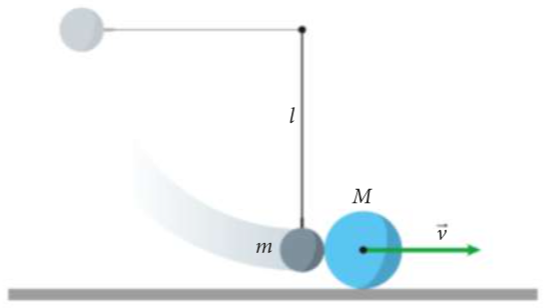
\includegraphics[width=0.23\textwidth]{images/pendolo-urto.png}
\end{wrapfigure}

\noindent
Il pendolo viene lasciato cadere dalla posizione orizzontale (\(\theta = 90^\circ\)) rispetto alla verticale.
Quando raggiunge la posizione verticale (\(\theta = 0^\circ\)), la sferetta urta \textbf{elasticamente} contro una biglia di massa \(M = 2{,}13 \, \text{kg}\) in quiete su un piano orizzontale.
La biglia parte con velocità \(v = 2{,}0 \, \text{m/s}\).

\medskip\noindent
Calcola la lunghezza \(l\) del pendolo.
\begin{solution}
    \textbf{Fase 1 — Velocità della sferetta alla posizione verticale.}

    Per la conservazione dell'energia meccanica (il pendolo scende di \(h = l\)):
    \[
        \frac{1}{2}m\,v_0^2 = m\,g\,l \implies v_0 = \sqrt{2gl}.
    \]

    \textbf{Fase 2 — Urto elastico sferetta–biglia.}

    Dalla formula per la velocità finale del secondo corpo in un urto elastico 1D:
    \[
        v = \frac{2m}{m+M}\,v_0 \implies v_0 = \frac{(m+M)\,v}{2m} = \frac{(1{,}0 + 2{,}13)\cdot 2{,}0}{2 \cdot 1{,}0} = \frac{3{,}13 \cdot 2{,}0}{2} = 3{,}13 \, \text{m/s}.
    \]

    \textbf{Fase 3 — Ricavo di \(l\).}
    \[
        v_0 = \sqrt{2gl} \implies l = \frac{v_0^2}{2g} = \frac{(3{,}13)^2}{2 \cdot 9{,}81} = \frac{9{,}797}{19{,}62} \approx 0{,}50 \, \text{m}.
    \]
\end{solution}
\end{question}
